\documentclass{article}
\usepackage{graphicx}
\usepackage[normalem]{ulem} % needed by strike
\usepackage[urlcolor=blue,colorlinks=true]{hyperref}
\usepackage[latin1]{inputenc}  % char encoding

\title{TXT2TAGS SAMPLE}
\author{Aurelio Jargas}
\begin{document}
\date{07/26/2008}
\maketitle
\clearpage


\section*{Introduction}
Welcome to the txt2tags sample file.

Here you have examples and a brief explanation of all
marks.

The first 3 lines of the this file are used as headers,
on the following format:

\begin{verbatim}
line1: document title
line2: author name, email
line3: date, version
\end{verbatim}

Lines with balanced equal signs = around are titles.


\section*{Fonts and Beautifiers}
We have two sets of fonts:

The NORMAL type that can be improved with beautifiers.

The TYPEWRITER type that uses monospaced font for
pre-formatted text.

We will now enter on a subtitle...

\subsection*{Beautifiers}
The text marks for beautifiers are simple, just as you
type on a plain text email message.

We use double *, /, - and \_ to represent \textbf{bold},
\textit{italic}, \sout{strike} and \underline{underline}.

The \textbf{\textit{bold italic}} style is also supported as a
combination.

\subsection*{Pre-Formatted Text}
We can put a code sample or other pre-formatted text:

\begin{verbatim}
  here    is     pre-formatted
//marks// are  **not**  ``interpreted``
\end{verbatim}

And also, it's easy to put a one line pre-formatted
text:

\begin{verbatim}
prompt$ ls /etc
\end{verbatim}

Or use \texttt{pre-formatted} inside sentences.

\subsection*{More Cosmetics}
Special entities like email (\htmladdnormallink{duh@somewhere.com}{mailto:duh@somewhere.com}) and
URL (\htmladdnormallink{http://www.duh.com}{http://www.duh.com}) are detected automagically,
as long as the horizontal line:


\hrulefill{}

\^{} thin or large v

\clearpage

You can also specify an \htmladdnormallink{explicit link}{http://duh.org}
with label.

And remember,

	\begin{quotation}
A TAB in front of the line does a quotation.
		\begin{quotation}
More TABs, more depth (if allowed).
		\end{quotation}
	\end{quotation}
Nice.


\section*{Lists}
A list of items is natural, just putting a \textbf{dash} or
a \textbf{plus} at the beginning of the line.

\subsection*{Plain List}
The dash is the default list identifier. For sublists,
just add \textbf{spaces} at the beginning of the line. More
spaces, more sublists.

\begin{itemize}
\item earth
  \begin{itemize}
  \item america
    \begin{itemize}
    \item south america
      \begin{itemize}
      \item brazil
      \item how deep can i go?
      \end{itemize}
    \end{itemize}
  \item europe
    \begin{itemize}
    \item lots of countries
    \end{itemize}
  \end{itemize}
\item mars
  \begin{itemize}
  \item who knows?
  \end{itemize}
\end{itemize}

The list ends with \textbf{two} consecutive blank lines.

\subsection*{Numbered List}
The same rules as the plain list, just a different
identifier (plus).

\begin{enumerate}
\item one
\item two
\item three
  \begin{itemize}
  \item mixed lists!
  \item what a mess
    \begin{enumerate}
    \item counting again
    \item ...
    \end{enumerate}
  \end{itemize}
\item four
\end{enumerate}

\subsection*{Definition List}
The definition list identifier is a colon, followed by
the term. The term contents is placed on the next line.

\begin{description}
\item[orange]
  a yellow fruit
\item[apple]
  a green or red fruit
\item[other fruits]
  \begin{itemize}
  \item wee!
  \item mixing lists
    \begin{enumerate}
    \item again!
    \item and again!
    \end{enumerate}
  \end{itemize}
\end{description}


\section*{Tables}
Use pipes to compose table rows and cells.
Double pipe at the line beginning starts a heading row.
Natural spaces specify each cell alignment.

\begin{center}\begin{tabular}{|l|c|r|}
\hline \textbf{heading 1} & \textbf{heading 2} & \textbf{heading 3} \\
\hline cell 1.1 & cell 1.2 & cell 1.3 \\
\hline cell 2.1 & cell 2.2 & cell 2.3 \\
\hline \end{tabular}\end{center}

Without the last pipe, no border:

\begin{center}\begin{tabular}{lcr}
\textbf{heading 1} & \textbf{heading 2} & \textbf{heading 3} \\
cell 1.1 & cell 1.2 & cell 1.3 \\
cell 2.1 & cell 2.2 & cell 2.3 \\
\end{tabular}\end{center}


\section*{Special Entities}
Because things were too simple.

\subsection*{Images}
The image mark is as simple as it can be: \texttt{[filename]}.

                      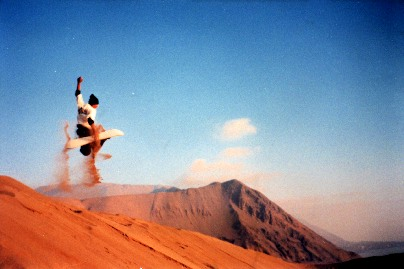
\includegraphics{img/photo.jpg}  

\begin{itemize}
\item The filename must end in PNG, JPG, GIF, or similar.
\item No spaces inside the brackets!
\end{itemize}

\subsection*{Other}
The handy \texttt{\%\%date} macro expands to the current date.

So today is 20080726 on the ISO \texttt{YYYYMMDD} format.

You can also specify the date format with the \%? flags,
as \texttt{\%\%date(\%m-\%d-\%Y)} which gives: 07-26-2008.

That's all for now.


\hrulefill{}


\includegraphics{img/t2tpowered.png} (\htmladdnormallink{sample.t2t}{sample.t2t})


% LaTeX2e code generated by txt2tags 2.5 (http://txt2tags.sf.net)
% cmdline: txt2tags -t tex samples/sample.t2t
\end{document}
